%Author Alex Clemmer, Landon Gilbert-Bland, Colton Meyers, Andrew Kuhnhausen
%CS 3505 Computer Organization
%Assignment 02:
\documentclass[a4paper]{article}
\usepackage[pdftex]{graphicx}
\usepackage{fancyvrb}
\usepackage{multirow}
\usepackage{amssymb}
\usepackage{amsmath}
\usepackage{fullpage}
\addtolength{\oddsidemargin}{-.05in}
	\addtolength{\evensidemargin}{-.05in}
	\addtolength{\textwidth}{.25in}

	\addtolength{\textheight}{.25in}
\begin{document}

\section*{CS 3505 Assignment 02}
Landon Gilbert-Bland\\
Andrew Kuhnhausen\\
Colton Meyers\\
Alex Clemmer\\

\section{Design Purpose}

The product we were meant to build was a spellchecker. There were several (artificial) design constraints in this assignment: we were required to use C++ implemented as per $\texttt{g++ v4.*}$, with all data structures (save a few notable exceptions, like $\texttt{string}$) to be completely hand-coded and managed. More notably, were also explicitly told to implement both a hash table and a BST, and to manage the memory properly.

\section{Implementation}

\subsection*{Basic timeline:}

Our first group meeting happened on the first Wednesday of the assignment, and lasted for roughly 3 hours. In this time, we came up with the meat of the algorithm we were implementing, as well as the API for the entire application. We created the API specifically by generating $\texttt{.h}$ files for every required file, as well as every file that we would need to implement the central algorithm.

Next came the one-time cost of developing the group's ``system". In this phase, we implemented a secure repository for our version control, as well as our code review platform, forums, wikis, and issue trackers.

Our next group meeting was Saturday. At this point, we had the base working (both the hash table and the BST), which left the implementation of the algorithm. The details of what we did are noted below. We also began the implementation of our testing framework in order to start testing our core classes.

We then divided the project up into as many independent tasks as we could find, which allowed us to each concentrate on something individually, and reduced our over all communications overhead by at least 50\%.

The next phase was the longest: the time was spent implementing everything. We spent at least 18 hours each doing this. We met both in pairs and as a group to complete the work, although some of it was done individually (depending on the task).

The last phase was testing, which we did extensively---although ``last" is misleading, because we implemented the Google Tests C++ testing framework about 3 days into the project. A lot of this phase rolls up into the last phase (it comprised probably 50\% or more of the implementation phase), but in addition to that, we spent probably 3 or 4 hours each (maybe even more) just doing pure testing.

$\textbf{NOTE that the details of our development strategy are under ``Reflections".}$ $\textbf{If you are}$ $\textbf{looking}$ $\textbf{for this}$ $\textbf{information, please see our (extensive) notes there.}$

\subsection*{Our goals:}

C++ is hard and introduces a lot of new things to learn. Our goals therefore mainly pertained to getting the project to work, rather than getting it to be the best spellchecker ever. (Consider that if we had to implement this in Java or Python or Ruby, the opposite would be the case.)

\begin{itemize}
	\item Implement and test required files ($\texttt{Dictionary}$, $\texttt{Word\_Count}$, $\texttt{Hashtable}$, $\texttt{BST}$, $\textit{et al}$)
	\item Catch 100\% of all errors as possible
	\item Make $\sim$30\% correct spelling suggestions.
	\item Finish before that Monday to leave room for testing.
\end{itemize}

Readers may be wondering why we only want a 30\% accuracy for corrections. This is because catching misspelled words is really easy, but suggesting them is really hard. Not only is the subject of ongoing research, even the experts tend to only get about 80\% on a good day. Consider that most people will probably base their algorithms on a certain infamous researcher's spell correction algorithm, but even that only gets 67\% correct on spelling suggestions for a reasonably good document.

\subsection*{Implementation:}
\subsubsection{The Problem:}

Corrections are harder than one would be inclined to think. Consider if I misspell the word $\textit{cow}$ with an 'h' instead of a 'w' ($\textit{i.e.}$, ``coh"), what is a machine supposed to correct this to? Let's just list all possible corrections considering $\textit{only}$ substitutions of the last letter: cob, cod, cog, con, coo, cop, cot, coy. Note that this list does not even consider substituting other letters or accounting for letters that we missed when typing this word, or letters that were added erroneously.

A reasonably good spellchecking mechanism therefore cannot use minimum edit distance. Instead, we will have to use some probabilistic mechanism to infer which words are correct. This is actually pretty open-ended problem, but considering the problems we had last time, we decided to keep it simple: we're going to make this decision almost entirely based on how likely a correction is to appear in the English language.

\subsubsection{The algorithm:}

Almost all implementations will begin by building a probabilistic model of English. You can accomplish this in a number of ways, but we chose just to look through a large corpus and count the number of times each word appears.

The base of this implementation are our $\texttt{File.cpp}$ and $\texttt{Hashtable.cpp}$ files. The first parses words out of the corpus and hashes each of them in a $\texttt{Hashtable}$. If the word is already in the table, the value at its key is incremented; if not, it's set to 1. This gives us a count (sort of like a histogram for the English language) that tells us roughly how often a word occurs. We can use this as the basis of our probabilistic inference.

To spellcheck a document we again call $\texttt{File.cpp}$ and parse the words in a file. Each word in turn is then subject to a combinatorial analysis. This was a point of contention but $\textbf{note that}$ $\textbf{under explicit}$ $\textbf{permission from}$ $\textbf{the instructor,}$ $\textbf{we did not}$ $\textbf{use a BST for this}$. Why? Even though we implemented the BST itself, using it to find misspellings was critically flawed for several reasons:

First, as we have seen above in the ``problems" section, minimum edit distance alone gets us nowhere. The other important thing to note is that it is also a really bad solution even in providing the words within a one-character edit distance, because although at each node you can branch off and try to spell a word using the ``wrong" letters one letter at a time ($\textit{i.e.}$, starting at the first letter of $\textit{cow}$ and walking down the tree to see if all possible permutations are correct, which would for example include starting with 'a' and seeing if $\textit{aow}$ and $\textit{bow}$ and $\textit{dow}$ and so on are all in the dictionary, and then repeating it for each letter in the word), one important thing that it's a $\textit{lot}$ harder to do is to account for if you missed a letter, or added one on top of the word.

So rather than implementing that inelegant and error-prone solution, we just decided to combinatorially figure out every possible word within a two-character edit distance that it could be and check to see if each is in the dictionary. This worked out pretty well.

Our suggestion is then the word that is ``most probable" based on our histogram hash table described above.

The other thing we should probably mention is that we implemented $\texttt{Word\_Count}$ with a self-sorting vector, rather than a hash table. The reason was because sorting the words as they were added made it loads easier to find the top $x$ results.

Another thing, for reference, is that we have included a multi-threaded $\texttt{Dictionary}$. We did this because our algorithm lends itself well to multithreading, but we do no use it as our core because our multithreading was so terrible that there was no advantage in speed. We could have fixed it, but we decided it wasn't worth it.


\subsection*{Where we were successful:}

Clear win for our first goal: we did not just implement all the requirements and get them functionally working, we actually implemented the Google Tests ($\texttt{gtests}$) C++ testing framework, and thoroughly tested our classes. You can view our tests in the $\texttt{tests/}$ and $\texttt{check\_file\_tests/}$. Our methodology is covered in the ``testing" section below.

Goal two is also pretty close to a win. We do find almost all words that are misspellings. The one sticking point is words that appear very infrequently in the English language. How do you train to accept words you haven't seen, and may never see? We have some answers, but we didn't have time to implement them, and the point is that it should work in the common case.

Goal three is a bit harder to judge. Depending on the document we use, on the linguistic complexity, on the domain we're working in, and so on, our accuracy ranges from 20-60\%. It is not obvious which metric to use, and thus it is not obvious this goal has been accomplished.

What is obvious is that our spellchecker (presumably like most of them) tends to do much better in common-path domains, or where words are used both common and consistent. This, of course, is expected.

These caveats in mind, we feel we were moderately successful at achieving goal three, although it could have been implemented with a lot more complexity.

Goal four was a clear win. We finished Monday night and spent most of the next few days either testing, relaxing, or thinking of ways to improve our application. See our bug reports a the bottom for proof of this.

\subsection*{Where we failed:}

There were several features that were not explicitly in our goals that we wanted to implement, but didn't. One important deficiency in our process---and this is due to a failure of communication---was word parsing. Data indicates that a lot of our misspellings are missed because our parsing scheme was poor. Getting word parsing exactly right is $\textit{very}$ hard, but our implementation is beyond naive: we really just stop parsing words at punctuation, which means a word like ``don't" would end up being ``don".

Another place we failed was probabilistic inference. Again, it's not that our mechanism doesn't work, but there are several things we could have done in order to make huge improvements to our suggestion ability. For example, consider that we are basically estimating the probability that a user meant some word $w_1$ given that they typed a ``bad" word, $b$: $P(w_1|b)$. Bayes' rule tells us that this is equivalent to $\cfrac{P(b|w_1)P(w_1)}{P(b)}$.

In other words, we can improve our suggestions by estimating the probability that we typed $b$ when we meant $P(w_1)$. There are subtle ways to do this, but we know it can be done.

\section{Project length}

Our automated logs indicate that we spent about 55 hours on this project total. We probably spent slightly more than this. As noted before, for each person we estimate 5 hours for planning, 15-18 hours for implementation, and 4 hours for testing.

\section{Testing:}

Our testing battery uses Google's $\texttt{gtest}$ framework. Our formal verification testing is pretty straightforward: we implemented a series of tests to make sure that our custom files behaved as we thought they should. In $\texttt{Hashtable}$, for instance, we tested adding lots of numbers to the table, then adding lots of unique numbers to the table, then adding all the same numbers to the table, and then to top it off, we tested how the size increases when we rehash.

We're relatively certain that the data structures are correct. What we're most uncertain about is the parsing. As we've noted before, parsing is a particularly difficult problem, and we don't expect to get it right, although we do expect to get it right enough.

We tested a lot on handwritten files designed to exploit possible sticking points. Those tests should be in $\texttt{file\_check\_tests/}$. We also tested over some larger documents, but mainly to make sure that the program didn't fail in any important way. For accuracy tests, we found that smaller tests are generally better (more effective, more portable, more controllable), and big tests are really best to verify what your small tests should be saying.

We actually ended up testing so well during implementation that our bugs in the formal testing phase tended to be bugs in our testing code, rather than with our core. Consider that we had 2 total bugs reported to the issue tracker for the master branch. If we had not been working in independent branches that could be merged at will, and we did not force code reviews, this would not have been the case; in fact, it's hard for us to think that this would have been possible at all committing to a central repository. This model of concurrent development and testing has worked out so well that we will be doing it for every project.

\subsubsection*{Memory Management}

One thing we were explicitly careful about testing was memory management. To test this, we included a print statement that fired off every time something was deleted; then when we deleted ($\textit{e.g.}$) the hash table, we could watch and make sure that all the things we needed to delete ended up being deleted. It's not the most repeatable test, but we understand that this is one of the harder problems for C++ programmers, so we're not that worried.

Our method for deletion was basically to delete everything allocated on the heap inside of a given data structure, and then to delete the data structure itself. We made sure to do this even in our hash table tests.

\section{Reflections:}

\subsection*{Our dev pipeline:}

Arguably more impressive than anything we wrote was how well the development process went. We basically wanted to eliminate as much of the communications overhead as was humanly possible, and to shorten the feedback cycle to the nub. We accomplished this using a few crucial technologies, which collectively proved to be extremely valuble.

\begin{itemize}
	\item $\textbf{Version control}$ We knew that VCSs were useful, but they become a lot more useful when a lot of people are working on a project. We are prepared to grant our very rapid pace of development as a product largely of two things: the ability to branch and merge our version history trivially, and to commit locally.
	
	In truth, these are the same thing: by being forced to commit to a local repository, rather than a central repository, our team members were able to experiment and checkin to their version control system freely without having to worry about breaking the build or introducing bugs for anyone else. And by being able to branch and merge trivially, our members were able to experiment with, and selectively discard changes they disliked. Using commands similar to $\texttt{cherry-pick}$, they were able to selectively put features into the central repository, which proved to be useful on several occasions.
	
	The ability to merge trivially meant that working on the same code was no longer a bottleneck, which meant greater code breathability and more familiarity with the codebase overall for all of our team members. All that's not to mention that we spent much more time developing software and much less time trying to get our VCS to merge, which we count as a huge win.
	
	\item $\textbf{Issue and bug tracking}$ Every time we introduced a bug or ran into a wall and needed a new feature, we put it up on the issue tracker. In this way, anyone could pick an issue and address it at their convenience. The difference between having a formal issue tracker and a glob of emails asking people to do things is like the difference between getting emails as a TA and having the Moodle ticket system, where TAs get assigned problems to address.
	
	One major advantage is that everything gets documented, and you can see at a glance where there are bugs, what needs work, and roughly where the problems in dev are. Another advantage is that people who need something to do just need to pick something out of a library of issues. Yet another advantage is that you can (and should) actually assign issues to people, which means that they usually get done.
	
	Here's a picture of some issues in our issue tracker:\\
	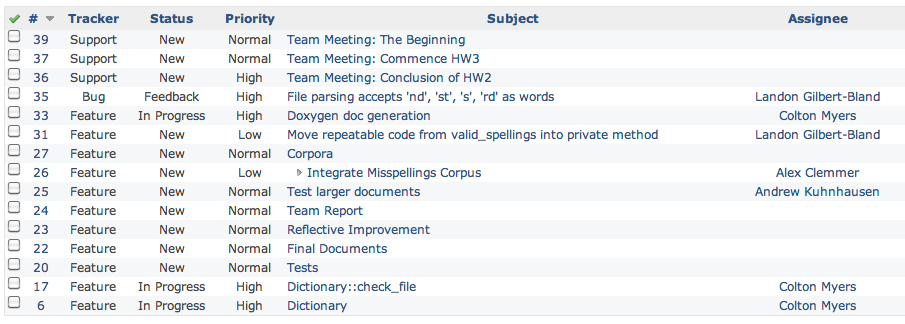
\includegraphics[scale=0.4]{issues.png}
	
	\item $\textbf{Code review}$ Implementing code review meant that two people had to sign off on every line of code that you wrote. This kept the code a reasonably good quality, first, because you knew you were being watched, and second, because we were able to catch everyone's stupid mistakes. Posting to code review was a simple unix command: $\texttt{post review --parent=master}$. Doing this put up the diff online, at which point members could look at what changed, comment on a line-by-line basis, and approve or reject it.
	
	The difference between doing this and emailing tarballs around, or even pulling the branch and looking at the diff yourself is unequivocal, and we want to be emphatic about it: we will never not use this tool again; it is invaluable in terms of time saved in communication and pulling branches alone. And that's to say nothing of the fact that it forces us to be thorough: since the review doesn't go away until it's approved or rejected, you have to address it at some point.
	
	One issue we will have to address in the future is the consistency of reviews. Andrew and Landon tended to issue reviews pretty quickly, but were often left hanging when their code needed a second review. This did cause a minor hiccup in the process, but it is easily corrected. 
	
	Here's a picture of someone commenting on a diff in review board:\\
	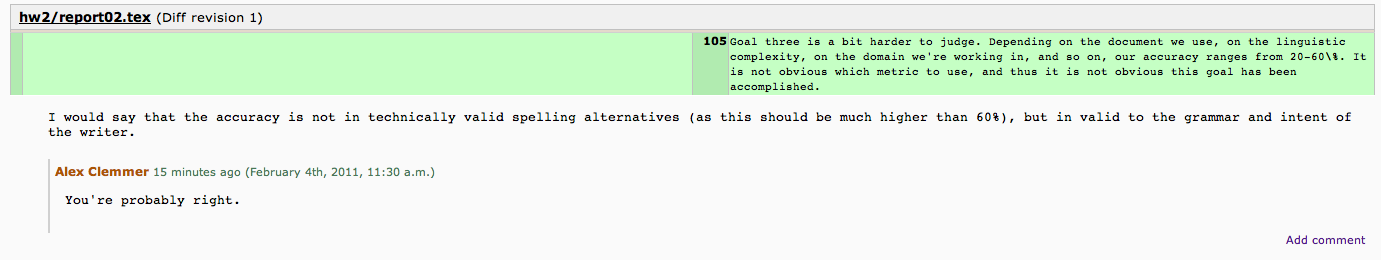
\includegraphics[scale=0.3]{review_board_diff.png}
	
	And here's a picture of a diff itself:\\
	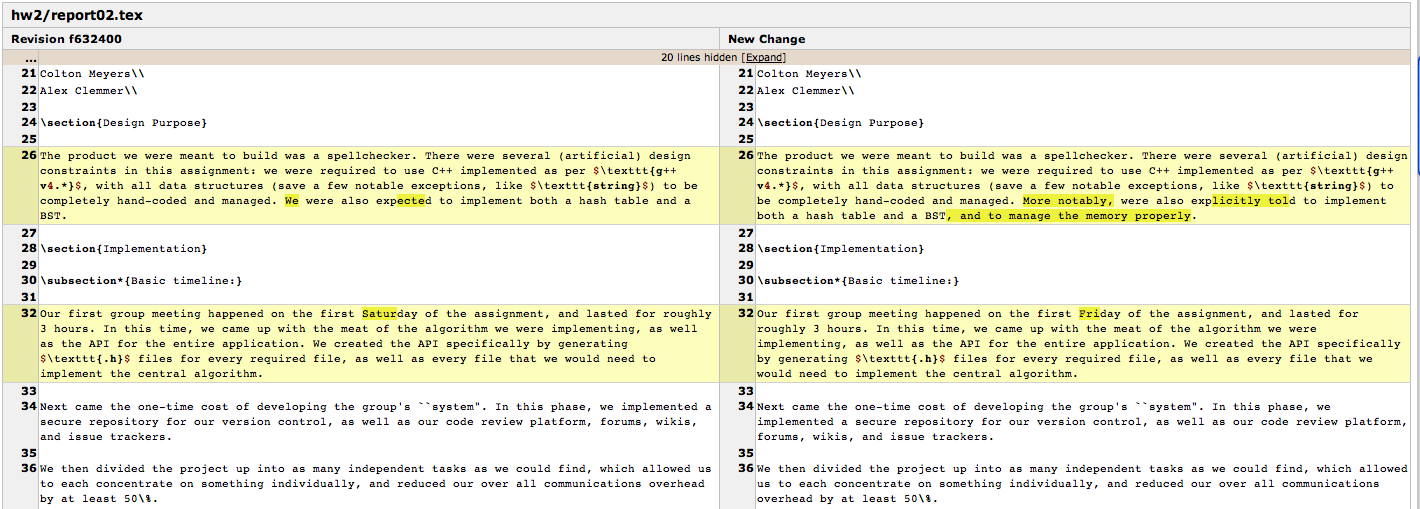
\includegraphics[scale=0.3]{review_board_diff2.png}
	
	\item $\textbf{Auto-wikis, auto-stats, and forums}$ We found that wikis increased our ability to document not just the code, but the process, while auto-stat analysis gave us a good idea of how the project was progressing, as well as choke points. Forums are good for addressing design problems.
	
	More importantly, it's useful to have these tasks divided into compartments designed to address them. This system is infinitely superior to a series of emails, both because accessibility and organization is trivial in comparison to searching through piles of old mail, and because everyone sees the same thing, rather than what's in their inbox.
	
	Here's a picture of our update tracker:\\
	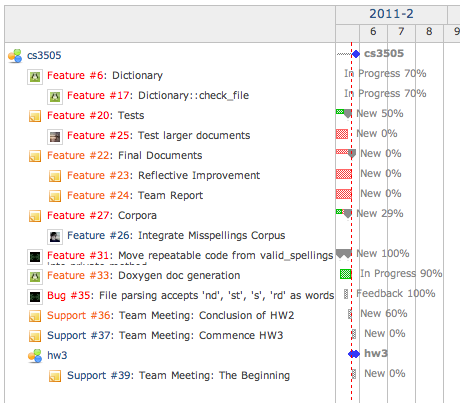
\includegraphics[scale=0.5]{update_calendar.png}
	
	Here's a shot of our wiki (talking about $\texttt{gtest}$ integration):\\
	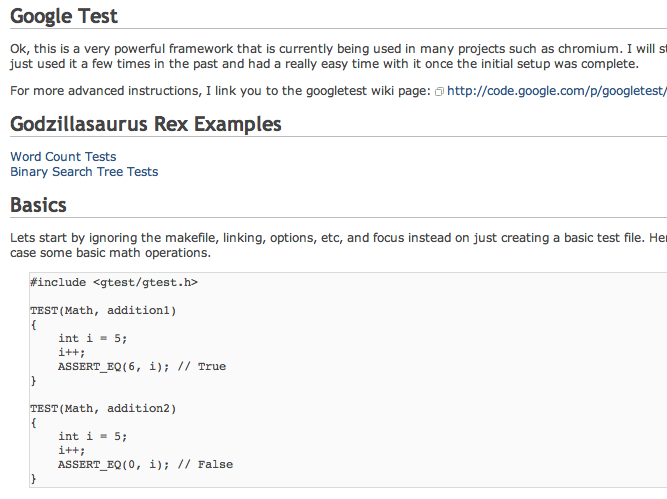
\includegraphics[scale=0.4]{wiki.png}
	
	Here is a helpful summation of our bugs in total:\\
	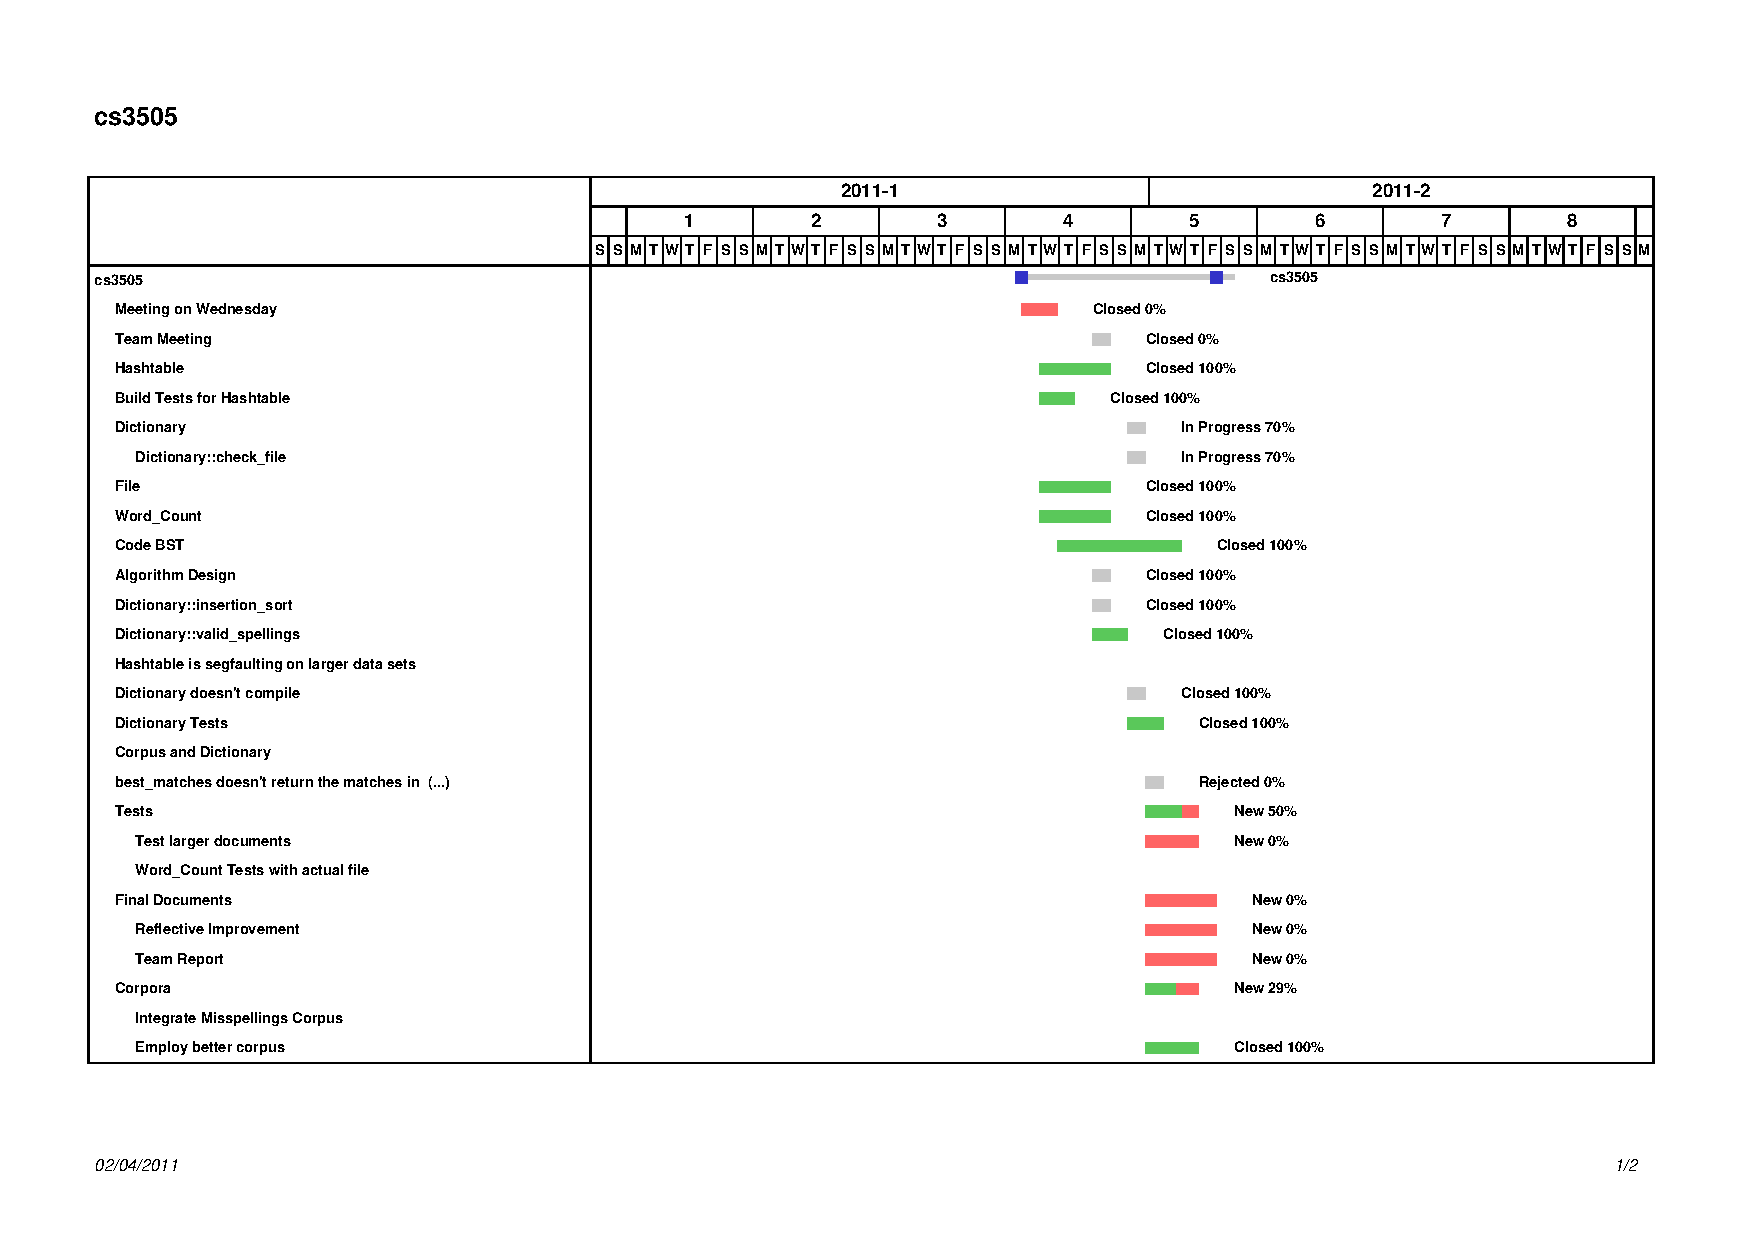
\includegraphics[scale=0.6]{cs3505-gantt.pdf}
	
	
\end{itemize}






























\end{document}